\chapter{Lecture 10: Residues and Poles} % Main chapter title

\begin{definition}
    [Residue]
    Suppose f is analytic on $0 < |z - z_0| < r$, if $0 < s < r$ Define the \textbf{\textit{residue of $f$ at $z_0$}} to be
    $$\text{Res}(f;z_0) = \frac{1}{2\pi i} \int_{|z - z_0| = s} f(z) dz$$
\end{definition}

\begin{remark}
    \textbf{\textit{Note:}} $\text{Res}(f; z_0)$ does not depend on $s$!
\end{remark}

\begin{theorem}
    [Green's Theorem] Suppose $f$ is analytic on $0 < |z - z_0| < r$, then
    $$\int_{|z - z_0| = s_1}f(\xi) d\xi = \int_{|z - z_0| = s_2}f(\xi) d\xi$$
\end{theorem}

\section{Computing Residues with Power Series}

\begin{theorem}

    Suppose $f(z)$ has a pole of order $m \geq 1 $ at $z_0$, then
    \begin{equation}
        f(z) = \frac{H(z)}{(z - z_0)^m}
    \end{equation}
    Where $H$ is analytic at $z_0$ and $H(z_0) \neq 0$ on $\{|z-z_0| < r\}$ and $H(z_0) \neq 0$.
    Expand $H(z)$ in a Laurent series about $z_0$:
    $$H(z) = \sum_{n=0}^{\infty} c_n(z - z_0)^n$$
    Then
    \begin{equation}
        \boxed{f(z) = \frac{c_0}{(z - z_0)^m} + \frac{c_1}{(z - z_0)^{m-1}} + \cdots + \sum_{k=m}^{\infty} c_k(z - z_0)^{k-m}}
        \label{eq:10.1}
    \end{equation}
    So we say:
    \begin{equation*}
        \text{Res}(f; z_0) = c_{m-1}
    \end{equation*}
    i.e.the coefficent of $\frac{1}{(z - z_0)}$ in the Laurent series of $f$ about $z_0$ (equation \ref{eq:10.1}).
\end{theorem}

\begin{example}
    Find the residue of:
    $$f(z) = \frac{e^z -1}{z^2} \quad \text{at} \quad z_0 = 0$$

    \textbf{Solution:} We know that:

    \begin{align*}
        e^z                 & = 1 + z + \frac{z^2}{2!} + \cdots = \sum_{n=0}^{\infty} \frac{z^n}{n!}           \\
        \frac{e^z - 1}{z^2} & = \frac{1}{z^2} + \frac{z}{2!} + \cdots = \sum_{n=0}^{\infty} \frac{z^{n-2}}{n!} \\
    \end{align*}
    So the residue is $c_{-1} = \frac{1}{1!} = 1$.
\end{example}

\begin{example}
    Find the residue of:
    $$ f(z) = \frac{z^2 + 3z -1}{z+2} \quad \text{at} \quad z_0 = -2$$

    \textbf{Solution:}
    Let $w = z + 2$, then $z = w - 2$ and $dz = dw$. So
    \begin{align*}
        f(w) & = \frac{(w-2)^2 + 3(w-2) - 1}{w} = \frac{w^2 - 4w + 4 + 3w - 6 - 1}{w} = \frac{w^2 - w - 3}{w} \\
             & = \frac{w^2}{w} - \frac{w}{w} - \frac{3}{w}                                                    \\
             & = w - 1 - \frac{3}{w}                                                                          \\
             & = \frac{-3}{z + 2} - 1 + z + 2
    \end{align*}
    So the residue is $c_{-1} = -3$.
\end{example}

\section{Laurent series}

\begin{definition}
    [Laurent Series]
    Suppose $f$ is analytic on $0 \leq r < |z - z_0| < R$, then $f$ has a \textbf{\textit{Laurent series}} about $z_0$.
\end{definition}

\begin{theorem}
    [Laurent Series]
    if $f$ is analytic on $0 \leq r < |z - z_0| < R$, then we can write $f(z)  = f_1(z) + f_2(z)$ where:
    \begin{enumerate}
        \item $f_1(z)$ is analytic on $\{|z - z_0| < R\}$ and has a power series expansion about $z_0$.
        \item $f_2(z)$ is analytic on $\{|z - z_0| < R\}$ and has a power series expansion about $\infty$.
    \end{enumerate}
    And:
    \begin{enumerate}
        \item $f_1(z) = \sum_{k=0}^{\infty} a_k(z - z_0)^n$
        \item $f_2(z) = \sum_{k=1}^{\infty} b_k(z - z_0)^{-n}$
    \end{enumerate}
    So we can write:
    \begin{equation}
        \boxed{f(z) = \sum_{k = -\infty}^{\infty} a_k(z - z_0)^n} \quad \text{Laurent Series}
    \end{equation}
    Where $a_k = b_k$ if $k < 0$.
    And the expression converges on $r < |z - z_0| < R$.
\end{theorem}

\begin{proof}
    Take $z : r < |z - z_0| < R$, and $r_1, R_1$ such that:
    $$r < r_1 < |z - z_0| < R_1 < R$$
    Then $f$ is analytic on $\{|z - z_0| < R_1\}$.
    As we can see from figure \ref{fig:laurent_series}, $C_1$ is a simple, closed, positively oriented curve in $\{|z - z_0| < R_1\}$, so we can apply Cauchy's theorem to get:
    \begin{align*}
        f(z) & = \frac{1}{2\pi i} \int_{C_1} \frac{f(\xi)}{\xi - z} d\xi                                                                                          \\
             & = \frac{1}{2\pi i} \int_{|\xi - z_0| = R_1} \frac{f(\xi)}{\xi - z_0} dz  - \frac{1}{2\pi i} \int_{|\xi - z_0| = r_1} \frac{f(\xi)}{\xi - z_0} d\xi \\
    \end{align*}
    \begin{align*}
        \Gamma = \{|\xi - z_0| = R_1\} \quad \text{and} \quad \gamma = \{|\xi - z_0| = r_1\}
    \end{align*}

    Now we use a trick!

    \begin{align*}
        \frac{1}{\xi - z} & = \frac{1}{\xi - z_0 -(z - z_0)} = \frac{1}{\xi - z_0} \frac{1}{1 - \frac{z - z_0}{\xi - z_0}} \\
    \end{align*}
    On $\Gamma = \frac{z - z_0}{\xi - z_0} < 1$  so:
    \begin{align*}
        \frac{1}{\xi - z} & =  \sum_{k=0}^{\infty}\frac{(z - z_0)^{k}}{(\xi - z_0)^{k+1}}
    \end{align*}
    And on $gamma$ we have:
    \begin{align*}
        \frac{1}{\xi - z} & =  -\sum_{k=1}^{\infty}\frac{(z - z_0)^{k}}{(\xi - z_0)^{k+1}}
    \end{align*}

    Thus:
    \begin{align*}
        f(z) & = \sum_{k=0}^{\infty} (z - z_0)^k \frac{1}{2\pi i} \int_{\Gamma = |\xi - z_0| = R_1} \frac{f(\xi)}{(\xi - z_0)^{k+1}} d\xi \\
             & - \sum_{k=0}^{\infty} (z - z_0)^{-k} \frac{1}{2\pi i} \int_{\gamma = |\xi - z_0| = r_1} \frac{f(\xi)}{(\xi - z_0)^k} d\xi
    \end{align*}
\end{proof}

\begin{figure}[h!]
    \centering
    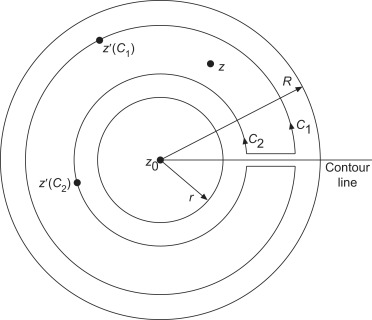
\includegraphics[width=0.7\textwidth]{LECTURE_10/laurent-series.jpg}
    \caption{Laurent Series}
    \label{fig:laurent_series}
\end{figure}

\begin{example}
    \begin{enumerate}
        \item $f(z) = \frac{H(z)}{(z - z_0)^m}$
        \item $f(z) = e^\frac{1}{z} = \sum_{n=0}^{\infty} \frac{z^{-n}}{n!}$
    \end{enumerate}
\end{example}